\documentclass[examenvragen.tex]{subfiles}

\begin{document}

\section{Matrix met dominante eigenwaarde}
\subsection{Opgave}
Gegeven de bijgevoegde Maple worksheet. Verklaar de grafieken. Wat is de orde van convergentie en de convergentiefactor? Wat zou er egebeuren als we in de methode geen normalisatie zouden gebruiken?

\subsection{Informatie}
\begin{itemize}
\item Boek hoofdstuk 6 deel 2: Het berekenen van eigenwaarden.
\item Boek pagina 290: Opmerking 5 (normalisatie)
\item Boek pagina 292: 6 Slotbemerkingen en samenvatting puntje 5 (convergentie- orde en factor)
\end{itemize}
\subsection{Antwoord}
In de Maple worksheet wordt de methode van de machten (met normalisatie) uitgevoerd op een matrix $A$ met een beginvector $x_0$
\[
A=
\begin{pmatrix}
9 & 1 & -1\\
0 & 10 & -5\\
0 & 0 & 8
\end{pmatrix}
\text{ en }
x_0 = \begin{pmatrix}
-1\\1\\1
\end{pmatrix}
\]
\[
x_{k} = A^{k}x_{0} 
\]
We berekenen eerst de eigenwaarden en eigenvectoren. De eigenwaarden vallen af te lezen op de diagonaal van $A$. Ze zijn re\"el en positief.
\[
\lambda_{1} = 10 \text{ en } E_{1} = \begin{pmatrix}1\\1\\0\end{pmatrix} 
\]
\[
\lambda_{2} = 9 \text{ en } E_{2} = \begin{pmatrix}1\\0\\0\end{pmatrix} 
\]
\[
\lambda_{3} = 8 \text{ en } E_{3} = \begin{pmatrix}-3\\5\\2\end{pmatrix} 
\]
De eigenvectoren vormen een en basis, dus $x_0$ kan uitgedrukt worden als een lineaire combinatie van de eigenvectoren $E_i$ met co\"efficienten $\alpha_i$.
\[
x_{0} = \alpha_{1}E_1 + \alpha_2E_2 + \alpha_{3}E_3
\]
We vinden voor deze $\alpha_i$ de volgende waarden.
\[
\alpha_1 = -\frac{3}{2} \text{, } \alpha_{2} = 2 \text{ en } \alpha_{3} = \frac{1}{2}
\]
Let op: $\alpha_1 \neq 0$. Dit is een voorwaarde om de methode van de machten te kunnen gebruiken. Controleer deze zeker!
We kunnen nu de uitdrukking voor $x_{k}$ uitwerken.
\[
x_{k} = A^{k}x_{0} = A^{k}(\alpha_{1}E_1 + \alpha_2E_2 + \alpha_{3}E_3) = (\alpha_{1}A^{k}E_1 + \alpha_2A^{k}E_2 + \alpha_{3}A^{k}E_3)
= \alpha_{1}\lambda_1^{k}E_1 + \alpha_2\lambda_2^{k}E_2 + \alpha_{3}\lambda_3^{k}E_3)
\]
\[
x_{k} = \lambda_{1}^{k}\left(\alpha_1E_1 + \left(\frac{\lambda_2}{\lambda_1}\right)^{k}\alpha_2E_2 + \left(\frac{\lambda_3}{\lambda_1}\right)^{k}\alpha_3E_3\right)
\]
In deze uitdrukking is $\lambda_{1}^{k}$ duidelijk dominant. Na voldoende iteraties zal er iets overblijven in $x_k$ van de volgende vorm.
\[
x_{k} = \lambda_{1}^{k}\alpha_1E_1 + o(1)
\]
In eerste Maple worksheet, wordt de eigenwaarde iteratief berekend met in de $j$-de iteratiestap $\lambda_{j}$. Dit zal inderdaad naar $\lambda_{1}$ convergeren.
\[
\lambda_{1_{j}} = \frac{\Vert x_{j}\Vert }{\Vert x_{j-1}\Vert}
\]
In de andere Maple worksheet zien we de relatieve fout. Deze verkleint zoals verwacht.

\subsubsection{Convergentiefactor}
De convergentiefactor berekenen we als $\frac{\lambda_{2}}{\lambda_{1}}$
\[
\rho = \frac{9}{10}
\]
We kunnen dit ook uit de grafiek aflezen.
\[
\epsilon_{40} = 10^{-2} \text{ en } \epsilon_{100} = 10^{-6}
\]
De verhouding van de fout in iteratiestap $j$ ten opzichte van de fout in iteratiestap $i$ is (ongeveer) de $j-i$-de macht van $\rho$.
\[
\rho^{100-40} \approx \frac{10_{-6}}{10^{-3}} = 10^{-3}
\]
\[
\rho \approx 0.89125
\]
\subsubsection{Convergentieorde}
De convergentiefactor is niet nul, en de fout daalt superlineair, dus de orde van convergentie is $1$. De methode van de machten convergeert lineair. Dit staat trouwens letterlijk in het boek op pagina 293.

\subsubsection{Zonder normalisatie}
Zonder normalisatie zou $x_{k}$ groeien als $O(n^{k})$. Dit zou vroeg of laat overloop met zich meebrengen. Dan valt er niets meer te zeggen over $\lambda_{1}$. Met normalisatie heeft $x_{k}$ steeds een lengte van $1$.

\iffalse
\paragraph{Gegeven:}
Maple afdruk: laatste vraag van de examenvragen in de winabundel (Die over het bepalen van eigenwaarden met de methode van de machten).\\
\\
Uit de matrix A = [2 1 -1; 0 3 -5; 0 0 -2] wordt de dominante eigenwaarde berekend. De startwaarden zijn: [-1.00001 1.00002 1]. Op de grafiek is zichtbaar dat er eerst naar 2 lijkt te convergeren, maar uiteindelijk toch de juiste eigenwaarde 3 gekozen wordt. Het berekenen gebeurt met de methode van de machten met normalisatie.
\paragraph{Gevraagd:}
\begin{itemize}
	\item Hoe komt het dat er eerst naar 2 geconvergeerd wordt?
	\item Waarom uiteindelijk toch naar 3?
	\item Wat als er geen normalisatie gebruikt zou worden?
\end{itemize}
\paragraph{Antwoord:}

We hebben gegeven: \\
$ A =\begin{bmatrix} 
 2 & 1 & -1 \\
 0 & 3 & -5 \\
 0 & 0 & -2\\
\end{bmatrix}$
$ X_0 = \begin{bmatrix}
-1.00001 \\
1.00002 \\
1 \\
\end{bmatrix} $ \\
De matrix A is een bovendriehoeksmatrix, dit wil zeggen dat we de eigenwaarden van A vinden op de hoofddiagonaal: $\lambda_1 = 2$,$\lambda_2 = 3$, $\lambda_3 = -2$. Hieruit leiden we af dat de dominante eigenwaarde 3 is. De methode van de machten zal dus normaal eerst naar de dominante eigenwaarde convergeren. Indien we de eigenvectoren van A berekenen, horende bij de eigenwaarden, dan vinden we: \\

$ E1 = \begin{bmatrix}
1 \\
0 \\
0 \\
\end{bmatrix} E2 = \begin{bmatrix}
1 \\
1 \\
0 \\
\end{bmatrix}  E3 = \begin{bmatrix}
0\\
1 \\
1 \\
\end{bmatrix}$ \\

(We berekenden deze eigenvectoren met de formule: $(A-\lambda I)=0$ ) voorbeeld voor $\lambda_1 = 2$:

$ A =\begin{bmatrix} 
 0 & 1 & -1 \\
 0 & 1 & -5 \\
 0 & 0 & -4\\
\end{bmatrix} \begin{bmatrix}
X_1 \\
X_2 \\
X_3 \\
\end{bmatrix} = \begin{bmatrix}
0 \\
0 \\
0 \\
\end{bmatrix} $ \\
We lossen dit stelsel op: \\
$-4X_3 = 0 $ \\
$X_2 - 5X_3 = 0 $ \\
$X_2 - X_3 = 0 $ \\
We merken op dat $X_1$ een vrije variabele is, voor de gemakkelijkheid stellen we deze gelijk aan 1 achteraf.
We krijgen dan: \\
$X_1 = 1 $ \\
$X_1 = X_3 = 0 $ \\
Wat ons de uitgekomen eigenvector E1 geeft. De werkwijze voor de overige 2 eigenvectoren is identiek. \\
We merken nu dat de startvector 
$ X_0 = \begin{bmatrix}
-1.00001 \\
1.00002 \\
1 \\
\end{bmatrix} $
ongeveer een lineaire combinatie is van de 2 eigenvectoren E1 en E3. Hierdoor zit de iteratie van het algoritme in het begin vast in het vlak van deze 2 eigenvectoren. Door de lichte afwijking op de vector (de .00001) komt de vector na genoeg iteraties toch uit het vlak en gaan we naar 3 itereren. Moest de startvector exact een lineaire combinatie van 2 eigen vectoren zijn dan zou men nooit naar 3 convergeren. (zie ook oefenzitting 10, Matlab sessie, daar hebben we ongeveer hetzelfde gedaan). De grafiek van de norm van de gevonden vector is ook gegeven en daar zie je dat hij eerst een tijd op 2 staat en dan pas na 20 stappen begint te schommelen en toch naar 3 gaat. Waarom? Omdat hij pas de afwijking van de ideale waarden (de .00001) gaat zien nadat de iteratieve methode de juiste precisie heeft bereikt. Dat wil zeggen na 20 stappen (1 stap is 1 bit en 3 bits per getal nauwkeurig $=>$ 20 stappen voor 6 getallen nauwkeurig). We maken gebruik van een genormaliseerde vorm om overloop of onderloop te vermijden. Door normalisatie gaat de norm van een vector namelijk beperkt zijn en is er dus minder kans op overloop/onderloop. De methode zal enkel naar $\lambda$ convergeren als $\lambda$ dominant is en de startvector een component heeft overeenkomstig met de eigenvector van $\lambda$. In de praktijk hang de bruikbaarheid van de von Mises methode af van de verhouding $\frac{| \lambda_2 |}{| \lambda_1 |}$ , de convergentiefactor. De methode kan falen om verschillende redenen: \\
\begin{itemize}
\item Startvector heeft geen component in de richting van de dominante eigenvector. (dit is als $\alpha$=0) In de praktijk zal dit probleem niet vaak voorkomen omdat afrondingsfouten vaak toch een component in die richting garanderen.
\item Er kunnen meerde eigenwaarden zijn met dezelfde (maximum) modules. De methode kan dan convergeren naar een lineaire combinatie van de overeenkomstige eigenvectoren.
\item Voor een re\"ele matrix en startvector, kan de methode nooit convergeren naar een complexe vector.
\end{itemize}
Zie ook vraag 4 van het opgeloste examen door van Barel zelf (ongeveer gelijke vraag).
\fi

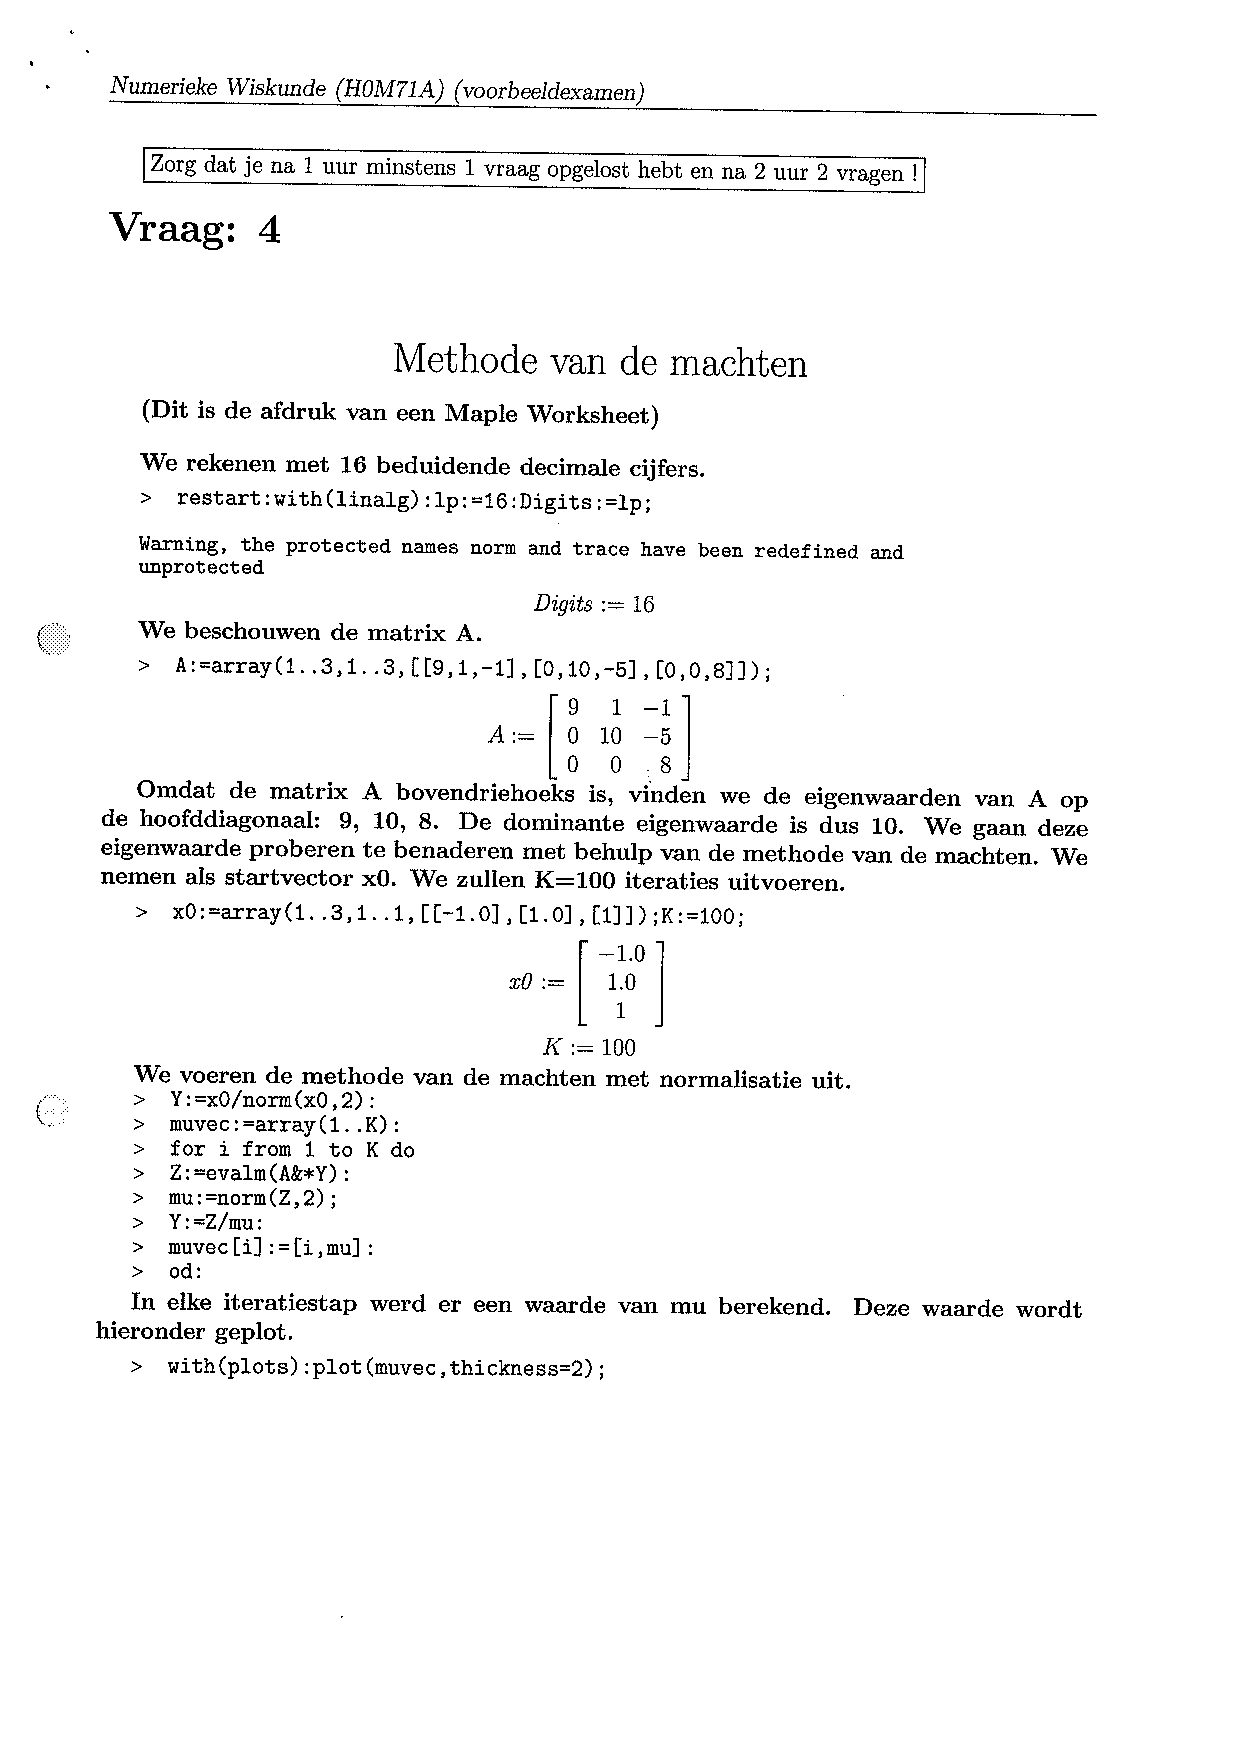
\includepdf[pages=-]{illustraties/vraag_matrix_met_dominante_eigenwaarde_maple_printout.pdf}
\end{document}
